\chapter{Analysis}

This section will look at the different steps in the process flow, what kind of input we expect, how the parsing is done and finally what kind of output we get. 

\section{Process flow}

Let's run the program and follow one SFS statute through the process flow to see what steps it goes through and how it changes. The statute chosen\footnote{The statute was chosen randomly, it does not have any specific properties that makes it more suitable as an example.} for this excerise is the \textit{Home guard regulation}\footnote{Hemvärnsförordningen \url{http://notisum.se/rnp/sls/sfs/20050819.pdf}} (1997:146). A transcript of the log created (when the 'debug' flag is turned on) during the parsing of this file can be found in the appendix, if the reader wants to follow the process steps.    

\subsection{Input files} 

The SFS statutes published in the Government Offices legal databases consists of two files for each statute, one \textit{Statute register file} (SFSR) and one \textit{Statute in full text} (SFST). The program expects the downloaded files to be saved in a specific tree structure to be able to read, create and save files.\\  

\begin{center}
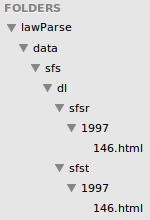
\includegraphics[scale=1]{../imgs/structure.png}
\captionof{figure}{Tree structure for downloaded files}
\end{center}
Under the root 'lawParse' there is a directory called 'data' which contains all different types of legal documents, here we have a 'sfs' directory where we store the downloaded, ('dl') parsed and eventually the generated files respectively. In all these directories we have another level for 'sfsr' and 'sfst' files, here the statutes are sorted according to the year they were created.        

\subsection{Parsing}

The first step is to scan the directory containing the files, this will give us a list of files, we will loop through the list one statute at the time. For our exampel (1997:146) statute we we will have the following set of files:\\ 
\begin{minted}[bgcolor=bg]{console}
All files connected to this file: 
	{'sfst': [u'../lawParse/data/sfs/dl/sfst/1997/146.html'], 
	 'sfsr': [u'../lawParse/data/sfs/dl/sfsr/1997/146.html']}
\end{minted}
\linebreak
We then transform and trim the file names so that they will be on the format '1997/146' instead of '../1997/146.html'. The actual parsing step then begins if the file met these three requirements:
\begin{enumerate}
\item If we have the file parsed already and it is newer than the incoming raw file, don't parse it again.
\item Filter out documents that are not proper SFS documents. They will have a name like ‘N1992:31’\footnote{It happens that other agencies publish documents to SFS, this is handled by giving them a SFS number preceded with an ‘N’}
\item Skip parsing the documents that have been or will be revoked, they are marked as \textit{“The constitution is repealed / shall be repealed”}\footnote{“Författningen är upphävd/skall upphävas”}
\end{enumerate}
The parsing begins with creating a SFS specific Parser, that has a set of properties and rules defined such as regular experssions created for parsing SFS statutes. Like this regular expression for matching a SFS number:\\
\begin{minted}[bgcolor=bg, firstline=2]{python}
$
reSimpleSfsId = re.compile(r'(\d{4}:\d+)\s*$')
\end{minted}
\linebreak
The raw string ('r') notation keeps the regular expression clean, without it every backslash would have to be prefixed with another on to escape it. Then we are looking for four (4) digits followed by a colon(:) and one (1) or more digits. The 's' at the end is there to match white spaces (behaves differently with or without the unicode flag turned on). Finally the dollar sign (\$) states that the match have to be the end of the string. The other regular expressions are created in a similar fashion, in total there are about 30 expression matching everything from chapter ids and numbered lists to the definition of a revoked date.\cite{regexpBib}\\\\  
When the SFSParser class is initialized and have all it’s properties created, we can divide the parsing into two steps. One where we handle the register file (SFSR) and one for the full text (SFST). We begin with creating a registry with \textit{registerposts} containing meta information and other information regarding changes to the statute.\\ 
\begin{minted}[bgcolor=bg]{python}
Registerpost: 
{u'Ansvarig myndighet': Link('u'Forsvarsdepartementet'',
	uri=u'http://lagen.nu/org/2008/forsvarsdepartementet'), 
 u'Ikraft': DateSubject(1997, 7, 1), 
 u'SFS-nummer': u'1997:146'}

Registerpost: 
{u'Omfattning': [
	u'andr. ', 
	Link('u'1 \xa7'',
	uri=u'http://rinfo.lagrummet.se/publ/sfs/1997:146#P1')],
 u'Ikraft': DateSubject(2012, 7, 16), 
 u'Rubrik': u'Forordning (2012:334) om andring i 
	hemvarnsforordningen (1997:146)', 
 u'SFS-nummer': u'2012:334'}
\end{minted}
\linebreak
\newline
The first registerpost created for 1997:146 describes basic properties such as responsible authority, entry into force and SFS number. The second\footnote{There's actually three register posts for 1997:146, I left a 'change post' out to save space} registerpost states that there has been some changes to the statute. We can find out if it is a change or if some part has been revoked\footnote{Omfattning can be for example "Change" or "Revoked" ("Ändr." or "Upph.")}, also we can see the force into entry and the change statute's SFS number. All these values are represented with different data types discussed in the 'Implementation' section, for ex. 'Link', 'DateSubject' or a unicode 'u' string.\\\\
The second part is to deal with the full text part of the statute, we do this by creating an intermediate text file with just the raw\footnote{It is not the complete downloaded file, we get rid of the "HTML" mark up of the document so that we only have text.} text. This file is saved in a directory called 'intermediate' on the same level as the downloaded, 'dl' directory in the file tree structure. \\\\ 
The file we have downloaded consist of a header with information similar to the register file. We could probably reuse some information\footnote{SFS number and responsible authority could be reused for example.} but we have everything set up for parsing and it is a fairly simple procedure so we go ahead and save it again. This information will be part of the header in the HTML file when that is created later on. For the information in the header we create a corresponding object, in the example below we create \textit{UnicodeSubjects}\footnote{We will look closer at this in the next section 'RDF markup'}, with the values \textit{SFS number} and \textit{Headline}, their predicates will be an URI to that object's definition.\\
\begin{minted}[bgcolor=bg]{python}
if key == u'Rubrik':
	meta[key] = UnicodeSubject(val, predicate=self.labels[key])
elif key == u'SFS nr':
	meta[key] = UnicodeSubject(val, predicate=self.labels[key])
\end{minted} 
\linebreak
\newline
Here is the values for the variables above when the header infromation is created:\\
\begin{minted}[bgcolor=bg]{console}
key:SFS nr
val:1997:146
self.labels[key]:
	http://rinfo.lagrummet.se/taxo/2007/09/rinfo/pub#fsNummer
key:Rubrik
val:Hemvarnsforordning (1997:146)
self.labels[key]:
	http://purl.org/dc/terms/title
\end{minted}
\linebreak
\newline
To mark up the full text we call a number of methods on the raw text file, to first of, find out what the part we are looking at should be represented as and then to create an object with that type's properties. The main method is \textbf{makeForfattning} when it is called it will in turn call several other methods like \textbf{makeKapitel,} \textbf{makeParagraf} and \textbf{makeTabell} and so on. The logic to figure out what each part should be marked up as uses a 'statehandler' to keep track of what part we just parsed and to guess what should come next. If we are inside the \textbf{makeStycke} method possible states/methods we can invoke are different types of lists and tables. Then when we reach the end of the current state we start over again and look what state the next part should be, this part can probably not be a list or a table, those states can only be reached from within certain states. Following that logic for example a paragraph can not be called within a chapter, each type has its place in the hierarchy. \\\\
All objects have an \textbf{"isObject"} and \textbf{"makeObject"} method, and they are for example used like the example below shows.\\ 
\begin{minted}[bgcolor=bg]{python}
def guesState(self):
	try:
		if self.reader.peekLine() == '':
			handler = self.blankLine
		elif self.isAvdelning():
			handler = self.makeAvdelning
		elif self.isKapitel():
			handler = self.makeKapitel
		elif self.isParagraf():
			handler = self.makeParagrafnd{minted}
		...
\end{minted}
\linebreak  
\newline
When we are done with the parsing the text body we add some additional information to the law’s meta information such as time created and preliminary work. To find out if there is any preliminary work we check the \textit{registerposts} in the register we have created, and save the URI to that document if existing.

\subsection{RDF markup }
During all the different parsing steps, I have mentioned that we create data objects with specialized properties for the different parts of the statute. Let's take a closer look at one of the objects that are created during our parse example.\\
In the previous section we look at example code for finding a statute's SFS number and headline, they are both of the type \textit{UnicodeSubject}. The class \textit{UnicodeSubject} it self does not do anything as we can see in the class definition below.\\
\begin{minted}[bgcolor=bg]{python}
class UnicodeSubject(PredicateType, UnicodeStructure):
	pass
\end{minted} 
\linebreak
\newline
However the class inherits from two other classes, \textit{PredicateType} and \textit{UnicodeStructure}. We are going to look at what our \textit{PredicateType} objects looks like. In the second chapter we stated that RDF is based upon the idea of making statements about resources in the form of triples of subject-predicate-object. Here we are obviously looking at the 'Predicate' part, as the class definition below reads; Inheriting from this class gives the child class a predicate attribute that describes the RDF predicate to which the class is the RDF subject.\\    
\begin{minted}[bgcolor=bg]{python}
class PredicateType(object):
    """Inheriting from this class gives the child class a 
    predicate attribute that describes the RDF predicate to 
    which the class is the RDF subject"""
    def __init__(self, *args, **kwargs):
	if 'predicate' in kwargs:
	    self.predicate = kwargs['predicate']
	    shorten = False
	    for (prefix, ns) in Util.ns.items():
		if kwargs['predicate'].startswith(ns):
		    predicateUri = kwargs['predicate']
		    kwargs['predicate'] = kwargs['predicate']
			.replace(ns, prefix + ':')	
		    shorten = True
		else:
		    from rdflib import RDFS
		    self.predicate = RDFS.Resource
	    super(PredicateType, self).__init__(*args, **kwargs)
\end{minted} 
\linebreak
\newline
When the object is initialized we compare the predicate's URI to some common name spaces that we have stored, if that is the case we can swap the long URI for a much shorter prefix. In our case with the SFS number and the title we can substitute the title's URI '\url{http://purl.org/dc/terms/title}' for simply 'dct:title' and '\url{http://rinfo.lagrummet.se/taxo/2007/09/rinfo/pub#fsNummer}' becomes 'rinfo:fsNummer'. Below we find part of the name space list, as we can see we can reuse definitions that are already defined by large international organisations, it is only 'rinfo' that is specific "Swedish-legal" definition.     
\begin{minted}[bgcolor=bg]{python}
# Common namespaces and prefixes for them
ns = {
    'dc':'http://purl.org/dc/elements/1.1/',
    'dct':'http://purl.org/dc/terms/',
    'rdfs':'http://www.w3.org/2000/01/rdf-schema#',
    'rdf':'http://www.w3.org/1999/02/22-rdf-syntax-ns#',
    'skos':'http://www.w3.org/2008/05/skos#',
    'rinfo':'http://rinfo.lagrummet.se/taxo/2007/09/rinfo/pub#',
    'xht2':'http://www.w3.org/2002/06/xhtml2/'
}
\end{minted} 
\linebreak
\newline
This way we can mark up our legal documents with short prefixes that makes the documents readable for both humans and computers in a way that contributes to the Semantic Web. In a final HTML file our title would look something like the snippet below, much more meaningful then just a header tag with a title, yet still simple enough to be understandable for human readers.\\
\begin{minted}[bgcolor=bg]{html}
<h1 property="dct:title">Hemvarnsforordning (1997:146)</h1>
\end{minted}
\linebreak
\newline
\subsection{Generating XHTML}
The way we are going to represent the parsed and marked up statute is as a XHTML file (in a later step we can transform the XHTML files to HTML to be able to display them to users in a browser). One of the reasons that the XHTML format is used is that through its extensibility and its focus on document structure it works well to represent legal documents in a semantically meaningful way.\\
To create an XHTML representation of the parsed statute we use a third party library called \textit{Genshi}\footnote{See the 'Implementation' section for more information regarding third party libs.}. We use Genshi's "TemplateLoader" to load a template we have created that specifies how we want our XHTML file to look like, ex. which values goes where etc. A nice feature with Genshi is that it uses a Stream-based filtering\footnote{\url{http://genshi.edgewall.org/wiki/Documentation/filters.html}} that allows us to apply various transformations as a template is being processed, without having to parse and serialize the output again.\\\\
Below is an example of how the template file renders a headline. As the code
snippet shows there is two <h> tag templates to chose from, one if it is a "normal" headline and one if it is an sub headline, then an extra class is added to the tag.\\
\begin{minted}[bgcolor=bg]{html}
<div py:def="render_rubrik(rubrik)" py:strip="" py:choose="">
    <h py:when="rubrik.type == 'underrubrik'" py:content="rubrik"
	id="${rubrik.id}" class="underrubrik">Underrubrik</h>
    <h py:otherwise="" py:content="rubrik"
	id="${rubrik.id}">Huvudrubrik</h>
</div>
\end{minted}
\linebreak  
\newline

\section{Output}
The output we get in form of a XHTML document consists of two parts a <head> and a <body> as normal HTML document. We are going to look at those parts\footnote{I will only show parts of the resulting XHTML document here to save space and to focus on some of the interesting parts. The full document can be found in the appendix.} to see what we ended up with after parsing and marking up our statute. \\\\
All documents will have several namespaces, they will be declared in the beginning of the document in the <html> element. These namespaces are mainly\footnote{The XHTML2 namespace is the default namespace and is used for elements and attributes.} used to express the predicate in the RDF triples that will be embedded in the document.\\ 
\begin{minted}[bgcolor=bg]{xml}
<?xml version="1.0" encoding="utf-8"?>
<html xmlns="http://www.w3.org/2002/06/xhtml2/" 
    xmlns:rdf="http://www.w3.org/1999/02/22-rdf-syntax-ns#" 
    xmlns:xsd="http://www.w3.org/2001/XMLSchema#" 
    xmlns:xsi="http://www.w3.org/2001/XMLSchema-instance" 
    xmlns:dct="http://purl.org/dc/terms/" 
    xmlns:rinfo="http://rinfo.lagrummet.se/taxo/2007/09/rinfo/pub#" 
    xmlns:rinfot="http://example.com/terms#" 
    xsi:schemaLocation="http://www.w3.org/2002/06/xhtml2/ 
    	http://www.w3.org/MarkUp/SCHEMA/xhtml2.xsd" 
    xml:base="http://rinfo.lagrummet.se/publ/sfs/1997:146" 
    xml:lang="sv" 
    about="http://rinfo.lagrummet.se/publ/sfs/1997:146">
\end{minted}
\linebreak
\newline

\subsection{Document head - metadata}
The first part of the document is inside the <head> element of the document, it contains metadata regarding the document. We find the obvious information such as title and a URI to rättsinformationsprojektet definition of the statute. Then further down there is some elements that are marked up with the RDFa\footnote{See chapter 2, section 2 regarding RDFa for more information about RDFa attributes} attributes. There are some that use the attributes “property” and “content” describing things such as SFS number and the date when the document was fetched. Lastly we find elements marked up with the “rel” (relationship) RDFa attribute, these are links to inter alia the change statutes we found for this statute.\\
\begin{minted}[bgcolor=bg]{html}
<head about="http://rinfo.lagrummet.se/publ/sfs/1997:146">
    <title>Hemvarnsforordning (1997:146)</title>
    <base href="http://rinfo.lagrummet.se/publ/sfs/1997:146"/>
    <link rel="rinfo:forfattningsamling" 
	href="http://rinfo.lagrummet.se/ref/sfs"/>
    <meta property="rinfo:fsNummer" content="1997:146"/>
    <meta property="rinfoex:senastHamtad" content="2012-08-01" 
	datatype="xsd:date"/>
    <meta property="rinfo:utfardandedatum" content="1997-04-10" 
	datatype="xsd:date"/>
    <link rel="rinfo:konsoliderar" 
	href="http://rinfo.lagrummet.se/publ/sfs/1997:146"/>
    <link rel="rinfo:konsolideringsunderlag" 
	href="http://rinfo.lagrummet.se/publ/sfs/1997:146"/>
    <link rel="rinfo:konsolideringsunderlag" 
	href="http://rinfo.lagrummet.se/publ/sfs/2005:819"/>
    <link rel="rinfo:konsolideringsunderlag" 
	href="http://rinfo.lagrummet.se/publ/sfs/2012:334"/>
</head>
\end{minted}
\linebreak
\newline

\subsection{Document body - Full text}
The second part of the document is the body, which consists of four parts itself, with the statute's title being the first.\\
\begin{minted}[bgcolor=bg]{html}
<h property="dct:title">Hemvarnsforordningen (1997:146)</h>
\end{minted}
\linebreak
It is a <h> tag (header) that is marked up with the RDFa attribute "property" which is set to "dct:title", meaning that this part is a title and the definition for title can be found using the namespace that "dct" is defined as in the beginning of the document\footnote{The prefix dct represents the Extended Dublin Core namespace}.\\\\
In XHTML it is possible to assign a role to an element, for example “contentinfo” or “main”\footnote{TODO: src}. This feature is used to declare that a certain section is the document’s actual text (main) etc. The next part of the body is marked with the role “contentinfo”. Which is including metadata relating to the document as a whole, and in the typical use case that should be visible to the user and not hidden in the document’s head. It can be thought of as a short intro with some short facts that the user might be interested in seeing right away when looking at the statute.\\
\begin{minted}[bgcolor=bg]{html}
<dl role="contentinfo">
...
<dt>SFS nr</dt>
    <dd property="rinfo:fsNummer">1997:146</dd>
<dt>Utgivare</dt>
    <dd rel="dct:publisher" 
	href="http://example.com/org/2008/regeringskansliet">
	Regeringskansliet</dd>
...
\end{minted}
\linebreak
\newline
As we can see from the figure above, the elements, SFS number and publisher are marked up with RDFa attributes.\\\\
The next section of the body is where it starting to get a little bit more interesting in a semantic point of view. It is the part with the documents actual text, it has been assigned the role “main”. If we look at the two first paragraphs below\footnote{The actual text includes åäö and "§" characters, but the latex plugin (minted) used to generate code snippets can not handle those characters, so I have manually removed them from this figure.}, we see that almost everything is marked up with RDFa attributes.\\
\begin{minted}[bgcolor=bg]{html}
<section role="main">
<h id="R1">Hemvarnets andamal</h>
<section id="P1" typeof="rinfo:Paragraf" about="#P1" 
    property="rinfot:paragrafnummer" content="1">
    <span rel="dct:isPartOf" 
	href="http://rinfo.lagrummet.se/publ/sfs/1997:146"/>
    
    <p id="P1S1" about="#P1S1" typeof="rinfo:Stycke">
    <span rel="dct:isPartOf" href="#P1"/>
    <span class="paragrafbeteckning">1</span>
    Hemvarnet har till uppgift att skydda skyddsobjekt. Hemvarnet 
    ska i ovrigt kunna stodja de operativa insatsforbanden och 
    delta i annan verksamhet dar Forsvarsmakten medverkar.
    </p>

    <p id="P1S2" about="#P1S2" typeof="rinfo:Stycke">
    <span rel="dct:isPartOf" href="#P1"/>
    Hemvarnet ingar i Forsvarsmakten.<a rel="dct:references" 
    href="http://rinfo.lagrummet.se/publ/sfs/1997:146#L2012:334">
    Forordning (2012:334).</a>
    </p>
</section>
...
</section>
\end{minted}
\linebreak
\newline
First we have a header with the id “R1” which stands for header number one\footnote{Rubrik in Swedish}. Then the first paragraph starts and that includes many RDFa attributes such as the “typeof” attribute which states that the following text is a paragraph and the definition for a paragraph can be found at the URI represented by “rinfo” followed by “Paragraf”. We can also see that this section has an id “P1”, which of course is short for “Paragraph one”. There is also a relation (the “rel” attribute), it is of the type “PartOf” which is a Dublin Core element, it is stating that this section is a part of the statute 1997:146. After that comes a similar code snippet but this time it is a “Stycke"\footnote{Stycke is a subsection or "subparagraph"} that is a part of “P1”, the first paragraph that is. It has the id “P1S1”, which stands for Paragraph one, Section one, this id notation continues by increasing the number for each element and concatenating sections as we traverse into the document tree.\\
The first paragraphs second section (P1S2) looks similar, it is marked up with a relation attribute with a reference to one of the change statutes (2012:819).\\\\
The last part of the document body is a section with the role “secondary”, as the name suggests it includes material that is not a part of the document text but is associated with it, typically a list of changes and transitions.\\
\begin{minted}[bgcolor=bg]{html}
<section role="secondary">
<h1>Andringar och overgangsbestammelser</h1>
...
<section id="L2012:334" 
    about="http://rinfo.lagrummet.se/publ/sfs/2012:334">
<dl>
<dt>Omfattning</dt>
    <dd>andr. <a rel="rinfo:ersatter"
    href="http://rinfo.lagrummet.se/publ/sfs/1997:146#P1">1</a></dd>
<dt>Ikraft</dt>
    <dd property="rinfo:Ikrafttradandesdatum">2012-07-16</dd>
<dt>Rubrik</dt>
    <dd property="dct:title">Forordning (2012:334) om andring i 
    hemvarnsforordningen (1997:146)</dd>
<dt>SFS-nummer</dt>
    <dd property="rinfo:fsNummer">2012:334</dd>
</dl>
</section>

    </section>
  </body>
</html>
\end{minted}
\linebreak
\newline
We can see that there is a section with the id “L2012:334” and a URI to that change statute. Then there is information regarding the change, what has been change, when is the entry into force date etc. All this information is of course marked up with RDFa attributes and elements from both the dct and rinfo namespaces. 
 
\subsection{RDF}
The vocabularies that are used are mainly, Dublin Core (dct) and Rättsinformationsprojekt's own vocabulary (rinfo). The Dublin Core vocabulary that is used is an extended version called “DCMI Terms”, some of the elements that are used from that are:\\ 
\begin{itemize}
\item \textbf{dct:title} - The document's title, for ex. "Hemvärnsförordningen" (1997:146)
\item \textbf{dct:publisher} - The publisher, for ex. “Regeringskansliet”
\item \textbf{dct:alternate} - A shorter prefix, ex “TF” for “Tryckfrihetsförordningen”
\item \textbf{dct:reference} - Used for references to another document. 
\end{itemize}
The other vocabulary, \textit{rinfo} is provided by Rättsinformationsprojektet\footnote{More information regarding Rättsinformationsprojektet's URI principles see \url{http://dev.lagrummet.se/dokumentation/system/uri-principer.pdf}}. It includes definitions such as "Ikrafttradandesdatum", "ersatter", "paragrafnummer" and other attributes that are specific to legal documents. A conceptual model that describes the document types, properties and other related matters that are Swedish Legal Information can be found in Rättsinformationsprojektet's documentation\footnote{Documentation in pdf format, \url{http://dev.lagrummet.se/dokumentation/model.pdf}}

\subsubsection{RDF Triples}
If we extract RDF data from the output document, which is possible with for example RDFa Distiller\footnote{RDFa Distiller \url{http://www.w3.org/2007/08/pyRdfa/}} we get all the RDF Triples for the document. Here are a couple of the resulting triples from the examples we have looked at earlier, displayed in N3-format.\cite{n3Bib}\\
\begin{minted}[bgcolor=bg]{xml}
<http://rinfo.lagrummet.se/publ/sfs/1997:146#P1S1> 
<http://purl.org/dc/terms/isPartOf>
<http://rinfo.lagrummet.se/publ/sfs/1997:146#P1>
...
<http://rinfo.lagrummet.se/publ/sfs/1997:146#P1S2>
<http://purl.org/dc/terms/references>
<http://rinfo.lagrummet.se/publ/sfs/1997:146#L2012:334>
\end{minted}
\linebreak
\newline
The first triple is stating that “P1S1 is a part of P1” that is, "Paragraph 1, Section 2" is a part of "Paragraph 1" which makes sense to a human reader but now it is also understandable to a computer. The second triple states that “P1S2 is a reference to L2012:334”, in this case, Paragraph 1, section 2 has been revoked and replaced with a new statute, 2012:334. With all these triples telling us about all sorts of things in our document, it also possible for computers to understand the meaning of the different parts, how they are connected and where to find more information about them.
\pagebreak
\section{Performance}
Even though performance is not the main focus of this thesis, it is still a part of it. As I stated in the problem statement, we are handling a lot of documents hence the program requires a fast process. The process has been tested on two computers\footnote{Note that I am not saying that the Mac is better than the Dell, I just happend to have a 2 years old Dell and a brand new Mac (also, the price differs with a about a factor of ten, so it should be faster no matter the brand.)} with quite different specifications, one pretty slow machine and one well above average (for a laptop). The result shows that the performance increases significantly\footnote{Almost all statutes parse in half the time on the Mac compared to the Dell} with a more powerful machine, which is positive since then it is not the case that the program itself is a limitation on how fast the process can run.\\\\
Computer specifications for benchmark:\\\\ 
\begin{tabular}{l l l}
\textbf{Make} & Dell & Apple\\
\textbf{Model} & Vostro V13 & MacBook Pro\\
\textbf{Processor} & Intel Celeron 743 @ 1.30 GHz & Intel Core i7 @ 2,6 GHz \\
\textbf{Memory} & 1.9 GB & 16 GB\\
\textbf{OS} & Ubuntu 12.04 32-bit & Mac OS X 10.8\\
\end{tabular}
\linebreak
\newline
To ensure that the performance is not disturbed by any other processes it has been run at night with all other programs shut down.\\

\subsection{Total running time}
As we can see from these numbers collected when running all SFS statutes\footnote{All the statutes that should be marked up, that is statutes that are valid i.e. not revoked. The total number of documents that pass through the process are about twice as many as the ones that get marked up, this time is negligible, but of course included in the total running time.} and what becomes even more clear in the charts below, most of the statutes are parsed and marked up very fast, the average running time on the mac is just above one second. There are a few statutes that are very slow that makes up most of the total running time.\\\\
\begin{tabular}{l l l}
\textbf{Computer} & \textbf{Dell Vostro} & \textbf{MacBook Pro}\\
Nr of statutes & 3424 & 3424\\
Average running time	& 2.53s & 1.06s\\
Max running time &  113.79s & 47.74s\\
Min running time & 0.97s & 0.40s\\
\textbf{Total running time} & 8700.59s / 2hrs 25min & 3721.26s / 1hrs 2 min\\
\end{tabular}
\linebreak
\newline
\subsection{Running time for selected statutes}
Because of the number of statutes I will only show a graph depicting the statutes from a few years (1942, 1967, 2005 and 2006)\footnote{These years are picked randomly, a couple more recent and a couple older years to get a good variation} to get a meaningful\footnote{Now the graph is showing 270 statutes, it would be impossible to include all ~3400 in a graph of this size.} graph. The purpose of the graph is to visualize that most statutes parse fast and few ‘heavy’ statutes comprise the majority of the time.\\\\
\begin{tabular}{l l l}
\textbf{Computer} & \textbf{Dell Vostro} & \textbf{MacBook Pro}\\
Nr of statutes & 270 & 270\\
Average running time	& 3.15s & 1.24s\\
Max running time &  71.98s & 28.71s\\
Min running time & 1.04s & 0.41s\\
\textbf{Total running time} & 860.59s & 337.79s\\
\end{tabular}
\linebreak
\newline
Below are the charts showing the statutes on the horizontal axis and the time in seconds on the vertical axis. The longer running times (blue) are from when the statutes were run on the Dell and the shorter ones (pink) on the Mac.\\\\ 
\includegraphics[scale=0.35]{../imgs/parseBoth.png}
\captionof{figure}{Chart showing running times for the selected statutes on both test computers}
\pagebreak
The statute that took the longest time\footnote{It is the forth statute from the left, partially covered by the vertical axis legend} (71.98s and 28.71s) is \textit{Rättegångsbalken} (1942:740) which consist of 59 chapters and more than 100 change statutes, hence it takes a lot of time to go through and mark up all that text.\\\\
In this next chart we have a zoomed in version of the chart with running times on the Mac for the selected statutes, here it becomes even more clear that most statuts parse very fast. As we can see that most statute's running time is less than two seconds (average running time is 1.24 seconds).\\\\
\includegraphics[scale=0.35]{../imgs/parseMac.png}
\captionof{figure}{Chart zoomed in to 6 seconds showing running times on the Mac for the selected statutes}

